%
%    This program is free software; you can redistribute it and/or modify
%    it under the terms of the GNU General Public License as published by
%    the Free Software Foundation; either version 2 of the License, or
%    (at your option) any later version.
%
%    This program is distributed in the hope that it will be useful,
%    but WITHOUT ANY WARRANTY; without even the implied warranty of
%    MERCHANTABILITY or FITNESS FOR A PARTICULAR PURPOSE.  See the
%    GNU General Public License for more details.
%
%    You should have received a copy of the GNU General Public License
%    along with this program; if not, write to the Free Software
%    Foundation, Inc., 675 Mass Ave, Cambridge, MA 02139, USA.
%

% Version: $Revision$

\section{Introduction}

Let $U=\{x_1,\ldots,x_n\}$, $n\ge 1$ be a set of variables.
%
A {\em Bayesian network} $B$ over a set of variables $U$ is a {\em
network  structure} $B_S$, which is a directed acyclic graph (DAG)
over $U$ and a set of  probability tables $B_P = \{p(u|pa(u)) | u\in
U\}$ where $pa(u)$ is the set of parents of $u$ in $B_S$. A Bayesian
network represents a probability distributions $P(U) = \prod_{u\in
U}p(u|pa(u))$.

Below, a Bayesian network is shown for the variables in the iris data set.
Note that the links between the nodes class, petallength and petalwidth 
do not form a {\em directed} cycle, so the graph is a proper DAG.

% information about screenshot
% - dataset: iris.arff
% - filter: weka.filters.unsupervised.attribute.Discretize -B 2 -M -1.0 -R first-last
% - classifier: weka.classifiers.bayes.BayesNet -D -Q weka.classifiers.bayes.net.search.local.TabuSearch -- -L 5 -U 10 -P 2 -S BAYES -E weka.classifiers.bayes.net.estimate.SimpleEstimator -- -A 0.5

\begin{center}
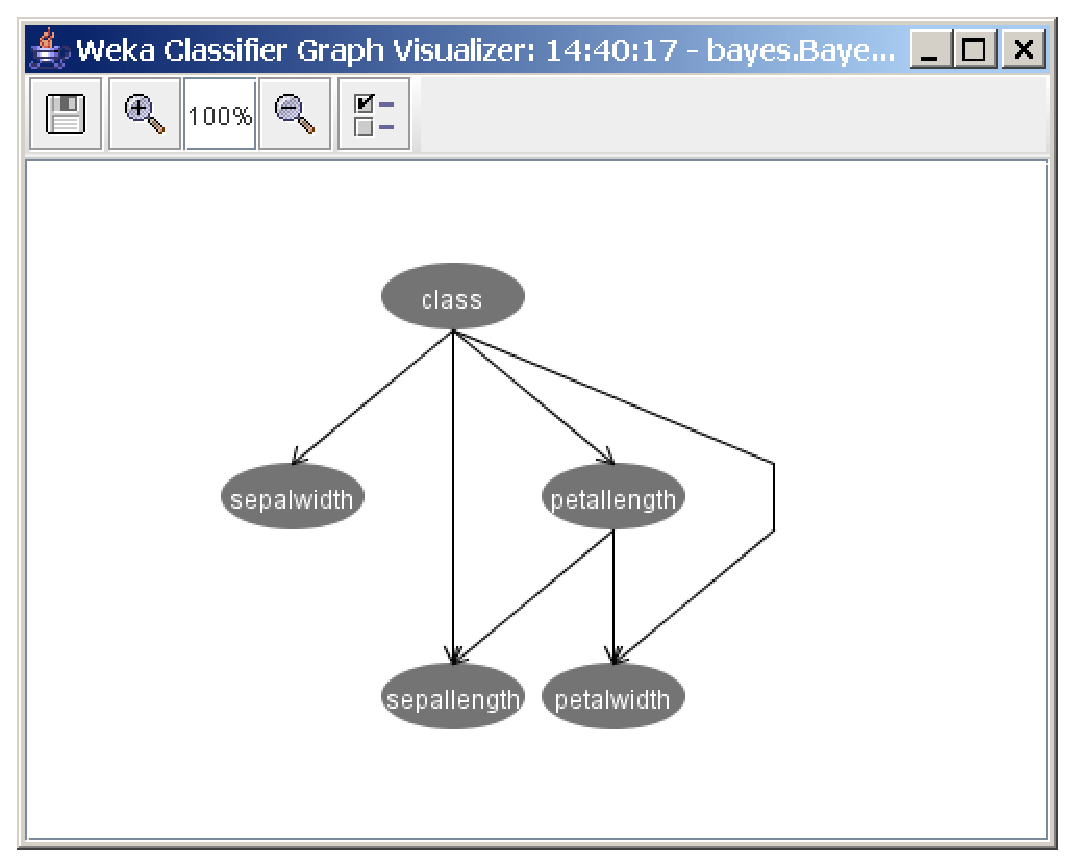
\epsfig{file=images/bayesnet/gui.net.eps,height=7cm}
\end{center}

This picture just shows the network structure of the Bayes net, but for
each of the nodes a probability distribution for the node given its parents
are specified as well. For example, in the Bayes net above there is a conditional distribution
for petallength given the value of class. Since class has no
parents, there is an unconditional distribution for sepalwidth.

\subsection*{Basic assumptions}

The classification task consist of classifying a 
variable $y=x_0$ called the {\em class variable} given a set of variables 
${\bf x} = x_1\ldots x_n$, called {\em attribute variables}. 
%For simplicity, only discrete finite variables with no missing values will be considered.
A classifier $h:{\bf x}\to y$
is a function that maps an instance of $\bf x$ to a value of $y$.
The classifier is learned from a dataset $D$ consisting of samples 
over $({\bf x}, y)$.
%
The learning task consists of finding an appropriate Bayesian network  
given a data set $D$ over $U$.  

All Bayes network algorithms implemented in Weka assume the following
for the data set:
\begin{itemize}
\item all variables are discrete finite variables. If you have a data set
with continuous variables, you can use the following filter to discretize them:\\
{\tt weka.filters.unsupervised.attribute.Discretize} 
\item no instances have missing values. If there are missing values in the
data set, values are filled in using the following filter:\\
{\tt weka.filters.unsupervised.attribute.ReplaceMissingValues}
\end{itemize}

The first step performed by {\tt buildClassifier} is checking if the data set fulfills
those assumptions. If those assumptions are not met, the data set is automatically
filtered and a warning is written to STDERR.\footnote{If there are missing values
in the test data, but not in the training data, the values are filled in in the
test data with a ReplaceMissingValues filter based on the training data.}

\subsection*{Inference algorithm}

To use a Bayesian network as a classifier, one simply calculates $argmax_yP(y|{\bf x})$
using the distribution $P(U)$ represented by the Bayesian network. 
Now note that

\begin{eqnarray}
P(y|{\bf x})&=&P(U)/P({\bf x})\nonumber\\
&\propto& P(U)\nonumber\\
&=&\prod_{u\in U}p(u|pa(u))\label{eq.infer}%\\
\end{eqnarray}

And since all variables in ${\bf x}$ are known, we do not need complicated inference
algorithms, but just calculate (\ref{eq.infer}) for all class values.

\subsection*{Learning algorithms}

The dual nature of a Bayesian network makes learning a Bayesian
network as a two stage process a natural division: first learn a
network structure, then learn the probability tables.

There are various approaches to structure learning and in Weka, the
following areas are distinguished:

\begin{itemize}
\item {\em local score metrics}: 
Learning a network structure $B_S$ can be considered an optimization
problem where a quality measure of a network structure given the
training data $Q(B_S|D)$ needs to be maximized. The quality measure
can be based on a Bayesian approach,  minimum description length,
information and other criteria. Those metrics have the practical property
that the score of the whole network can be decomposed as the sum 
(or product) of the score of the individual nodes. This allows for 
local scoring and thus local search methods.

\item {\em conditional independence tests}:
These methods mainly stem from the goal of uncovering causal structure.
The assumption is that there is a network structure that exactly represents
the independencies in the distribution that generated the data. Then it
follows that if a (conditional) independency can be identified in the data
between two variables that there is no arrow between those two 
variables. Once locations of edges are identified, the direction of the edges
is assigned such that conditional independencies in the data are properly
represented.

\item {\em global score metrics}:
A natural way to measure how well a Bayesian network performs on a
given data set is to predict its future performance by estimating
expected utilities, such as classification accuracy.  Cross-validation
provides an out of sample evaluation method to facilitate this by
repeatedly splitting the data in training and validation sets.  A
Bayesian network structure  can be evaluated by estimating the
network's parameters from the training set and the resulting Bayesian
network's performance determined against the validation set.  The
average performance of the Bayesian network over the validation sets
provides a metric for the quality of the network.

Cross-validation differs from local scoring metrics  in that the quality
of a network structure often cannot be decomposed in the scores of the
individual nodes. So, the whole network needs to be considered in order
to determine the score.

\item {\em fixed structure}:
Finally, there are a few methods so that a structure can be fixed, for
example, by reading it from an XML BIF file\footnote{See {\sf
\url{http://www-2.cs.cmu.edu/\~fgcozman/Research/InterchangeFormat/}{}}
for details on XML BIF.}.
\end{itemize}

For each of these areas, different search algorithms are implemented in 
Weka, such as hill climbing, simulated annealing and tabu search.

Once a good network structure is identified, the conditional probability
tables for each of the variables can be estimated.

You can select a Bayes net classifier by clicking the classifier 'Choose' button in 
the Weka explorer, experimenter or knowledge flow and find {\tt BayesNet}
under the {\tt weka.classifiers.bayes} package (see below).

\begin{center}
\epsfig{file=images/bayesnet/select.eps,height=7cm}
\end{center}

The Bayes net classifier has the following options:

\begin{center}
\epsfig{file=images/bayesnet/bayesnet.options.eps,height=7cm}
\end{center}

The {\tt BIFFile} option can be used to specify a Bayes network stored in
file in BIF format. When the {\tt toString()} method is called after learning the
Bayes network, extra statistics (like extra and missing arcs) are printed 
comparing the network learned with the one on file.

The {\tt searchAlgorithm} option can be used to select a structure learning
algorithm and specify its options.

The {\tt estimator} option can be used to select the method for estimating the
conditional probability distributions (Section \ref{sec.estimate}).

When setting the {\tt useADTree} option to \textbf{true}, counts are calculated using the
ADTree algorithm of Moore \cite{Moore}. Since I have not noticed a lot of 
improvement for small data sets, it is set off by default.
Note that this ADTree algorithm is different from the ADTree classifier algorithm
from {\tt weka.classifiers.tree.ADTree}.

The {\tt debug} option has no effect.

\section{Local score based structure learning\label{sec.score}}

Distinguish score metrics (Section 2.1) and search algorithms (Section 2.2).
A local score based structure learning can be selected by choosing one in the
{\tt weka.classifiers.bayes.net.search.local} package.

\begin{center}
\epsfig{file=images/bayesnet/local.algorithms.eps,height=8cm}
\end{center}


Local score based algorithms have the following options in common:\\
{\tt initAsNaiveBayes} if set {\bf true} (default), the initial network structure used
for starting the traversal of the search space is a naive Bayes network 
structure. That is, a structure with arrows from the class variable to
each of the attribute variables.\\
If set {\bf false}, an empty network structure will be used (i.e., no arrows at all).\\
{\tt markovBlanketClassifier} (\textbf{false} by default) if set {\bf true},
at the end of the traversal of the search space, a heuristic is used
to ensure each of the attributes are in the Markov blanket of the 
classifier node. If a node is already in the Markov blanket (i.e., is
a parent, child of sibling of the classifier node) nothing happens,
otherwise an arrow is added.\\
If set to {\bf false} no such arrows are added.\\
{\tt scoreType} determines the score metric used (see Section 2.1
for details). Currently, K2, BDe, AIC, Entropy and MDL are implemented.\\
{\tt maxNrOfParents} is an upper bound on the number of parents of each of the
nodes in the network structure learned.

\subsection{Local score metrics \label{sec.score.metric}}

We use the following conventions to identify counts in the database
$D$ and a network structure $B_S$.  Let $r_i$ ($1\le i\le n$) be the
cardinality of $x_i$.  We use $q_i$ to denote the cardinality of the
parent set of $x_i$ in $B_S$,  that is, the number of different values
to which the parents of $x_i$ can be  instantiated.  So, $q_i$ can be
calculated as the product of cardinalities of nodes in $pa(x_i)$,
$q_i=\prod_{x_j\in pa(x_i)}r_j$.  Note $pa(x_i)=\emptyset$ implies
$q_i=1$.
%
 We use $N_{ij}$ ($1\le i\le n$, $1\le j\le q_i$) to denote the number
of records in $D$ for which $pa(x_i)$ takes its $j$th value.%
We use $N_{ijk}$ ($1\le i\le n$, $1\le j\le q_i$, $1\le k\le r_i$) to
denote the number of records in $D$ for which $pa(x_i)$ takes its
$j$th value and for which $x_i$ takes its $k$th value.
%
So, $N_{ij}=\sum_{k=1}^{r_i}N_{ijk}$.  We use $N$ to denote the number
of records in $D$.

Let the {\em entropy metric} $H(B_S,D)$ of a network structure and database
be defined as
\begin{equation}\label{eq.H}
 H(B_S,D)=-N\sum_{i=1}^n\sum_{j=1}^{q_i}\sum_{k=1}^{r_i}\frac{N_{ijk}}{N}\log\frac{N_{ijk}}{N_{ij}}
\end{equation}
and the {\em number of parameters} $K$ as
\begin{equation}\label{eq.K}
K=\sum_{i=1}^n(r_i-1)\cdot q_i
\end{equation}

{\bf AIC metric} The AIC metric $Q_{AIC}(B_S,D)$ of a Bayesian network
structure $B_S$ for a database $D$ is
\begin{equation}\label{eq.AIC}
Q_{AIC}(B_S,D) = H(B_S,D)+K
\end{equation}
A term $P(B_S)$ can be added \cite{bouck1995} representing prior
information  over network structures, but will be ignored for
simplicity in the Weka implementation.

%{\bf RIC metric} The Risk Inflation Criterion (RIC) metric $Q_{RIC}(B_S,D)$ is
%\begin{equation}\label{eq.AIC}
%Q_{RIC}(B_S,D) = H(B_S,D)+log(K)
%\end{equation}
% NOTE: CANNOT DECOMPOSE INTO LOCAL SCORING METRIC

{\bf MDL metric} 
The minimum description length metric $Q_{MDL}(B_S,D)$
of a Bayesian network structure $B_S$ for a database $D$ is
is defined as

\begin{equation}\label{eq.MDL}
Q_{MDL}(B_S,D) = H(B_S,D)+\frac{K}{2}\log N
\end{equation}

{\bf Bayesian metric}
The Bayesian metric of a Bayesian network structure $B_D$ for a database $D$ is
$$
Q_{Bayes}(B_S,D) = P(B_S)\prod_{i=0}^n\prod_{j=1}^{q_i}\frac{\Gamma(N_{ij}')}{\Gamma(N_{ij}'+N_{ij})}
\prod_{k=1}^{r_i}\frac{\Gamma(N_{ijk}'+N_{ijk})}{\Gamma(N_{ijk}')}
$$
where $P(B_S)$ is the prior on the network structure (taken to be constant hence ignored 
in the Weka implementation) and $\Gamma(.)$ the gamma-function. $N_{ij}'$ and $N_{ijk}'$
represent choices of priors on counts restricted by 
$N_{ij}'=\sum_{k=1}^{r_i}N_{ijk}'$. With $N_{ijk}'=1$ (and thus $N_{ij}'=r_i$), 
we obtain the K2 metric \cite{CooperHerskovits1992}
$$
Q_{K2}(B_S,D) = P(B_S)\prod_{i=0}^n\prod_{j=1}^{q_i}\frac{(r_i-1)!}{(r_i-1+N_{ij})!}
\prod_{k=1}^{r_i}N_{ijk}!
$$
With $N_{ijk}'=1/r_i\cdot q_i$ (and thus $N_{ij}'=1/q_i$), we obtain the {\bf BDe metric}
\cite{heckerman95}.


\subsection{Search algorithms \label{sec.score.search}}

The following search algorithms are implemented for local score metrics;
\begin{itemize}
\item \textit{K2} \cite{CooperHerskovits1992}: 
hill climbing add arcs with a fixed ordering of variables.\\
Specific option: {\tt randomOrder} if {\bf true} a random ordering of
the nodes is made at the beginning of the search. If {\bf false} (default)
the ordering in the data set is used. The only exception in both cases is that
in case the initial network is a naive Bayes network ({\tt initAsNaiveBayes}
set \textbf{true}) the class variable is made first in the ordering.
\item \textit{Hill Climbing} 
\cite{Buntine1996}: 
hill climbing adding and deleting arcs with no fixed ordering of variables.\\
{\tt useArcReversal} if \textbf{true}, also arc reversals are consider when determining
the next step to make.
\item \textit{Repeated Hill Climber} starts with a randomly generated network and
then applies hill climber to reach a local optimum. The best network found is
returned.\\
{\tt useArcReversal} option as for Hill Climber.
\item \textit{LAGD Hill Climbing} does hill climbing with look ahead on a limited set of 
best scoring steps, implemented by Manuel Neubach. The number of look ahead steps and number of steps considered
for look ahead are configurable.
\item \textit{TAN} \cite{ChengGreiner1999,friedman97}:
\textit{T}ree \textit{A}ugmented \textit{N}aive Bayes where the tree is formed by calculating the
maximum weight spanning tree using Chow and Liu algorithm \cite{chow1968}.\\
No specific options.
\item \textit{Simulated annealing} \cite{bouck1995}:
using adding and deleting arrows.\\
The algorithm randomly generates a candidate network $B_S'$ close to the current
network $B_S$. It accepts the network if it is better than the current, i.e.,
$Q(B_S',D) > Q(B_S,D)$. 
Otherwise, it accepts the candidate with probability 
$$e^{t_i \cdot(Q(B_S',D) -Q(B_S,D))}$$
where $t_i$ is the temperature at iteration $i$.
The temperature starts at $t_0$ and is slowly decreases with each iteration. 

\begin{center}
\epsfig{file=images/bayesnet/score.sa.eps,height=5cm}
\end{center}

Specific options:\\
{\tt TStart} start temperature $t_0$.\\
{\tt delta} is the factor $\delta$ used to update the temperature, so $t_{i+1}=t_i \cdot \delta$.\\
{\tt runs} number of iterations used to traverse the search space.\\
{\tt seed} is the initialization value for the random number generator.\\

\item \textit{Tabu search} \cite{bouck1995}:
using adding and deleting arrows.\\
Tabu search performs hill climbing until it hits a local optimum.
Then it steps to the least worse candidate in the neighborhood. However,
it does not consider points in the neighborhood it just visited in the
last $tl$ steps. These steps are stored in a so called tabu-list.

\begin{center}
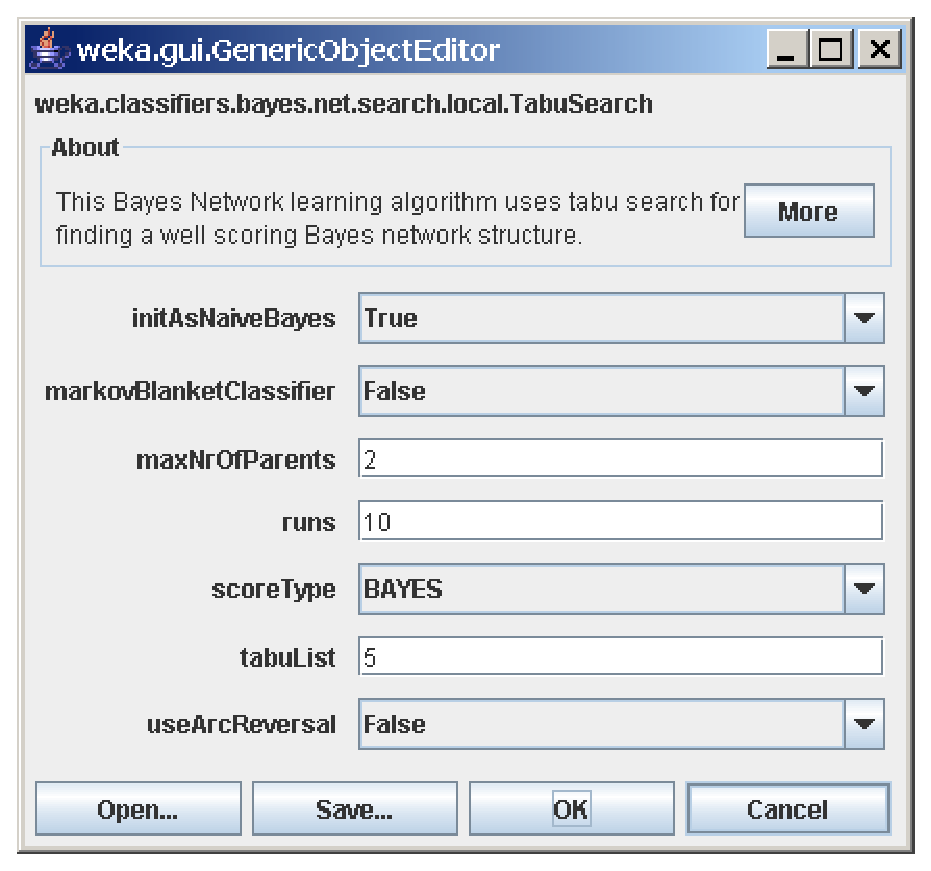
\epsfig{file=images/bayesnet/score.tabu.eps,height=5cm}
\end{center}

Specific options: \\
{\tt runs} is the number of iterations used to traverse the search space.\\
{\tt tabuList} is the length $tl$ of the tabu list.

\item \textit{Genetic search}: applies a simple implementation of a genetic search algorithm
to network structure learning. A Bayes net structure is represented by a array
of $n\cdot n$ ($n$ = number of nodes) bits where bit $i\cdot n + j$ represents whether
there is an arrow from node $j\to i$.\\

\begin{center}
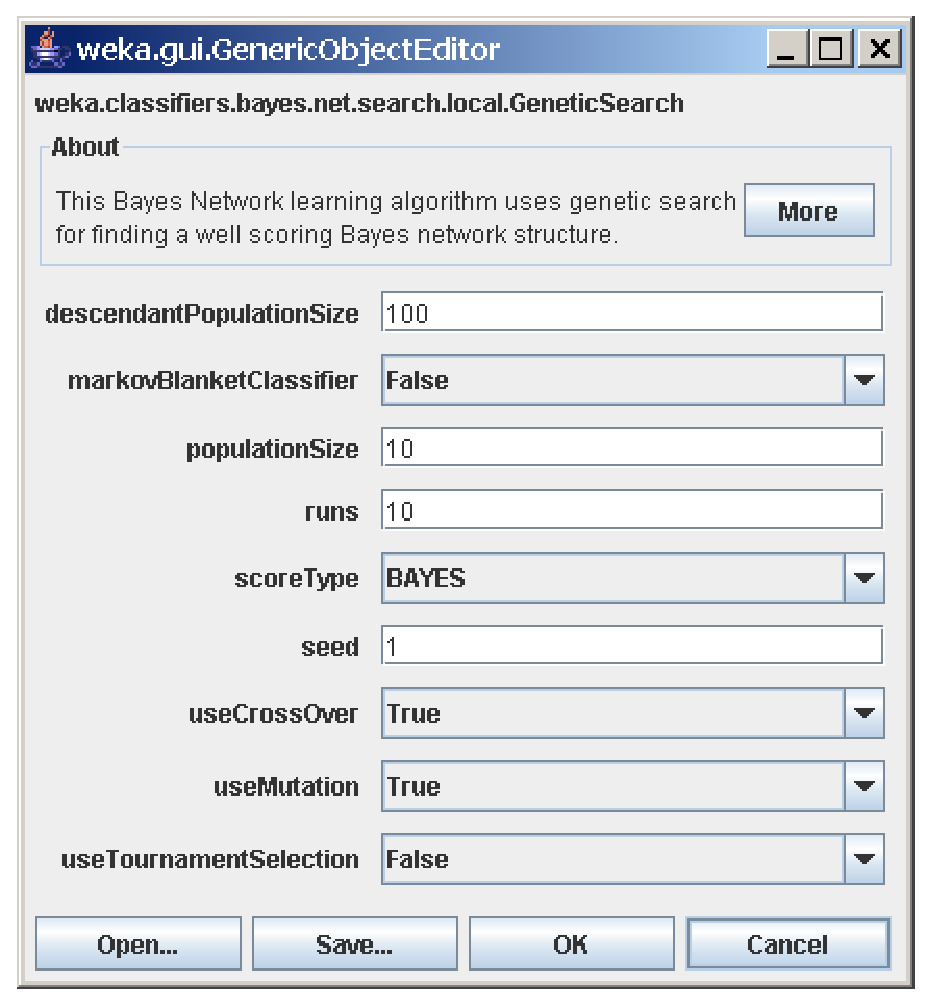
\epsfig{file=images/bayesnet/score.genetic.eps,height=8cm}
\end{center}

Specific options:\\
{\tt populationSize} is the size of the population selected in each generation.\\
{\tt descendantPopulationSize} is the number of offspring generated in each generation.\\
{\tt runs} is the number of generation to generate.\\
{\tt seed} is the initialization value for the random number generator.\\
{\tt useMutation} flag to indicate whether mutation should be used. Mutation is applied by
randomly adding or deleting a single arc.\\
{\tt useCrossOver} flag to indicate whether cross-over should be used. Cross-over is applied
by randomly picking an index $k$ in the bit representation and selecting the first $k$ bits
from one and the remainder from another network structure in the population.
At least one of \texttt{useMutation} and \texttt{useCrossOver} should be set to \textbf{true}.\\
{\tt useTournamentSelection} when \textbf{false}, the best performing networks are selected from
the descendant population to form the population of the next generation. 
When \textbf{true}, tournament selection is used. Tournament selection randomly chooses two
individuals from the descendant population and selects the one that performs best.\\
\end{itemize}

\section{Conditional independence test based structure learning}

Conditional independence tests in Weka are slightly different from the
standard tests described in the literature. To test whether variables
$x$ and $y$ are conditionally independent given a set of variables $Z$,
a network structure with arrows $\forall_{z\in Z}z \to y$ is compared with
one with arrows $\{x\to y\} \cup \forall_{z\in Z}z \to y$. 
A test is performed by using any of the score metrics described in Section 
2.1.

\begin{center}
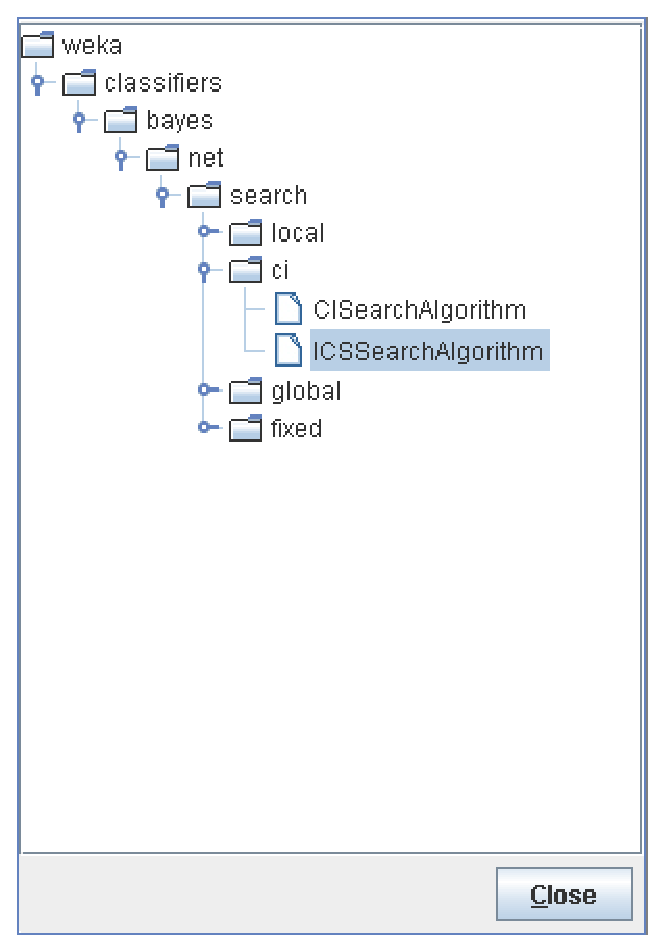
\epsfig{file=images/bayesnet/ci.algorithms.eps,height=8cm}
\end{center}

At the moment, only the ICS  \cite{verma}and CI algorithm are implemented. 

The ICS algorithm makes two steps, first find a skeleton (the undirected graph with edges $iff$ there
is an arrow in network structure) and second direct all the edges in the skeleton
to get a DAG.

Starting with a complete undirected graph, we try to find conditional independencies
$\langle x,y|Z\rangle$ in the data. For each pair of nodes $x$, $y$, we consider sets
$Z$ starting with cardinality $0$, then $1$ up to a user defined maximum. Furthermore,
the set $Z$ is a subset of nodes that are neighbors of both $x$ and $y$. If an
independency is identified, the edge between $x$ and $y$ is removed from the skeleton.

The first step in directing arrows is to check for every configuration $x--z--y$
where $x$ and $y$ not connected in the skeleton whether $z$ is in the set $Z$ of
variables that justified removing the link between $x$ and $y$ (cached in the
first step). If $z$ is not in $Z$, we can assign direction $x\to z\leftarrow y$.

Finally, a set of graphical rules is applied \cite{verma} to direct the remaining
arrows.
\begin{verbatim}
           Rule 1: i->j--k & i-/-k => j->k
           Rule 2: i->j->k & i--k => i->k
           Rule 3  m
                         /|\
                        i | k  => m->j
                i->j<-k  \|/
                          j
        
           Rule 4  m
                         / \
                        i---k  => i->m & k->m
                  i->j   \ /
                          j
           Rule 5: if no edges are directed then take a random one (first we can find)
\end{verbatim}

The ICS algorithm comes with the following options.

\begin{center}
\epsfig{file=images/bayesnet/ci.ics.eps,height=5cm}
\end{center}

Since the ICS algorithm is focused on recovering causal structure, instead of 
finding the optimal classifier, the Markov blanket correction can be made 
afterwards.\\
\\
Specific options:\\
The {\tt maxCardinality} option determines the largest subset of $Z$ to be 
considered in conditional independence tests $\langle x,y|Z\rangle$. \\
The {\tt scoreType} option is used to select the scoring metric.

\section{Global score metric based structure learning}

\begin{center}
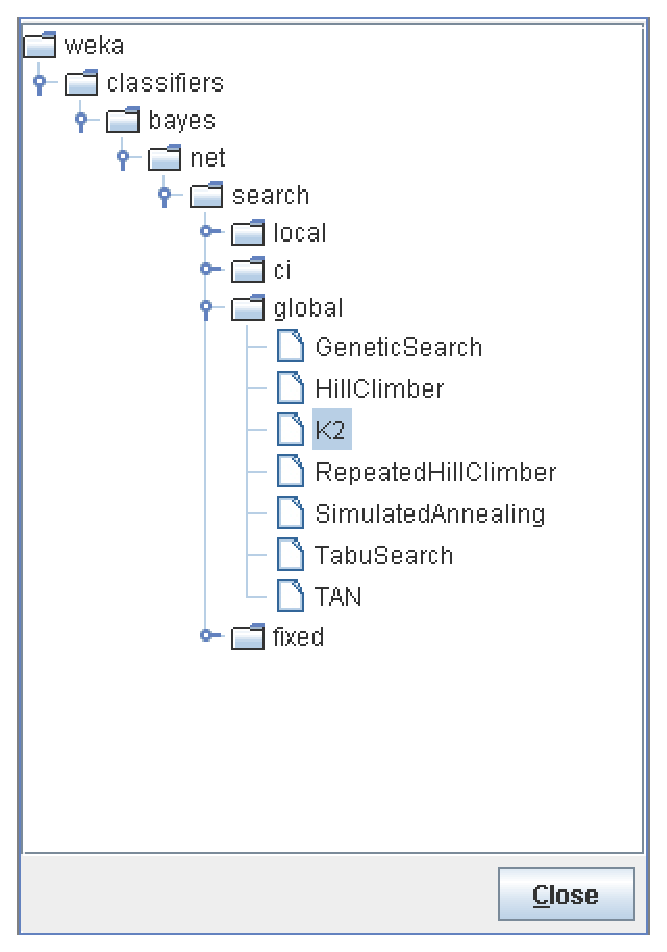
\epsfig{file=images/bayesnet/global.algorithms.eps,height=8cm}
\end{center}

Common options for cross-validation based algorithms are: \\
{\tt initAsNaiveBayes}, {\tt markovBlanketClassifier} and {\tt maxNrOfParents}
(see Section \ref{sec.score} for description).

Further, for each of the cross-validation based algorithms the {\tt CVType} can be
chosen out of the following:

\begin{itemize}
\item {\em Leave one out cross-validation (loo-cv)} selects $m=N$ training sets 
simply by taking the data set $D$ and removing the $i$th record for training 
set $D_i^t$. The validation set consist of just the $i$th single record. 
Loo-cv does not always produce accurate performance estimates. 

\item {\em K-fold cross-validation (k-fold cv)} splits the data $D$ in $m$ approximately 
equal parts $D_1,\ldots,D_m$. Training set $D_i^t$ is obtained by removing part 
$D_i$ from $D$. Typical values for $m$ are 5, 10 and 20. With $m=N$, k-fold cross-validation becomes loo-cv. 

\item {\em Cumulative cross-validation (cumulative cv)} starts with an empty data
set and adds instances item by item from $D$. After each time an item is added
the next item to be added is classified using the then current state of the
Bayes network.
\end{itemize}

Finally, the {\tt useProb} flag indicates whether the accuracy of the classifier
should be estimated using the zero-one loss (if set to {\bf false}) or using
the estimated probability of the class.

\begin{center}
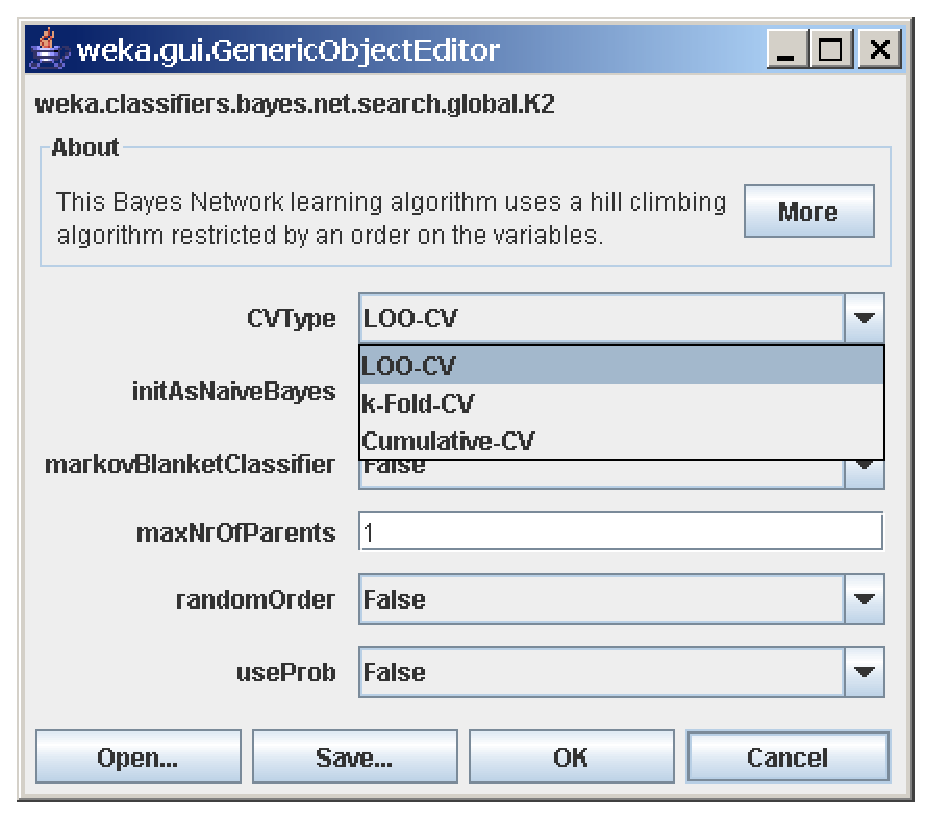
\epsfig{file=images/bayesnet/global.k2.eps,height=6cm}
\end{center}

The following search algorithms are implemented: K2, HillClimbing, RepeatedHillClimber,
TAN, Tabu Search, Simulated Annealing and Genetic Search. See Section \ref{sec.score} for
a description of the specific options for those algorithms.

\section{Fixed structure 'learning'}

The structure learning step can be skipped by selecting a fixed network
structure. There are two methods of getting a fixed structure: just make
it a naive Bayes network, or reading it from a file in XML BIF format.

\begin{center}
\epsfig{file=images/bayesnet/fixed.algorithms.eps,height=8cm}
\end{center}

\section{Distribution learning\label{sec.estimate}}

Once the network structure is learned, you can choose how to learn the probability
tables selecting a class in the {\tt weka.classifiers.bayes.net.estimate} package.

\begin{center}
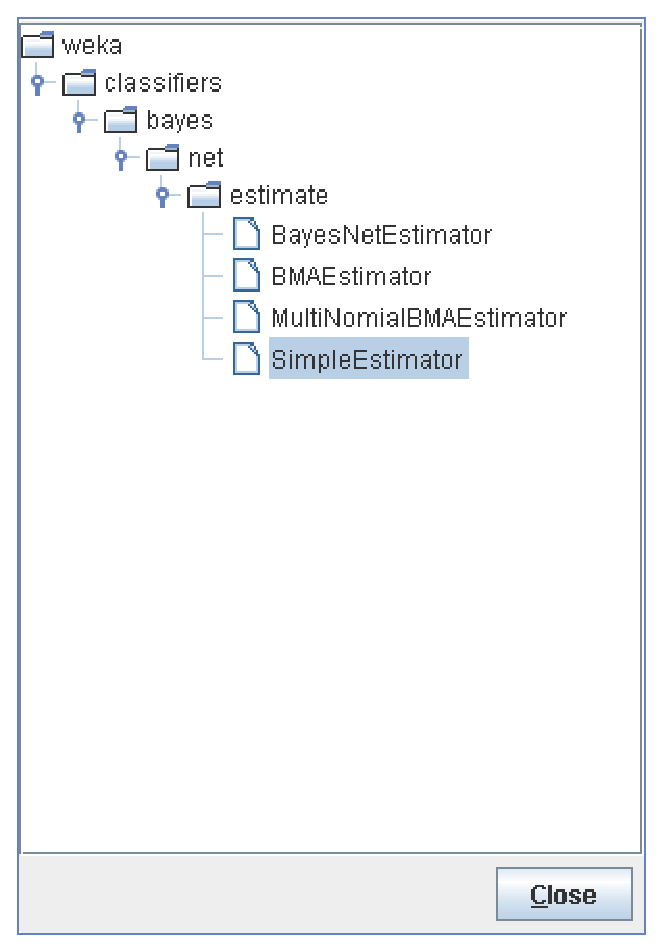
\epsfig{file=images/bayesnet/estimate.algorithms.eps,height=8cm}
\end{center}


The \texttt{SimpleEstimator} class produces direct estimates of the conditional probabilities,
that is, 
$$P(x_i=k|pa(x_i)=j)=\frac{N_{ijk}+N_{ijk}'}{N_{ij}+N_{ij}'}$$ 
where $N_{ijk}'$ is the alpha parameter that can be set and is
$0.5$ by default. With $alpha=0$, we get maximum likelihood estimates.

\begin{center}
\epsfig{file=images/bayesnet/estimate.direct.eps,height=4cm}
\end{center}

With the \texttt{BMAEstimator}, we get estimates for the conditional probability tables based
on Bayes model averaging of all network structures that are substructures of the
network structure learned \cite{bouck1995}. This is achieved by estimating the
conditional probability table of a node $x_i$ given its parents $pa(x_i)$ as a weighted 
average of all conditional probability tables of $x_i$ given subsets of $pa(x_i)$.
The weight of a distribution $P(x_i|S)$ with $S\subseteq pa(x_i)$ used is proportional
to the contribution of network structure $\forall_{y\in S}y\to x_i$ to either the
BDe metric or K2 metric depending on the setting of the {\tt useK2Prior} option (\textbf{false}
and \textbf{true} respectively).

\begin{center}

\epsfig{file=images/bayesnet/estimate.bma.eps,height=5cm}
\end{center}

\section{Running from the command line}
These are the command line options of {\tt BayesNet}.

{\small
\begin{verbatim}
General options:

-t <name of training file>
        Sets training file.
-T <name of test file>
        Sets test file. If missing, a cross-validation will be performed on the 
        training data.
-c <class index>
        Sets index of class attribute (default: last).
-x <number of folds>
        Sets number of folds for cross-validation (default: 10).
-no-cv
        Do not perform any cross validation.
-split-percentage <percentage>
        Sets the percentage for the train/test set split, e.g., 66.
-preserve-order
        Preserves the order in the percentage split.
-s <random number seed>
        Sets random number seed for cross-validation or percentage split
        (default: 1).
-m <name of file with cost matrix>
        Sets file with cost matrix.
-l <name of input file>
        Sets model input file. In case the filename ends with '.xml',
        the options are loaded from the XML file.
-d <name of output file>
        Sets model output file. In case the filename ends with '.xml',
        only the options are saved to the XML file, not the model.
-v
        Outputs no statistics for training data.
-o
        Outputs statistics only, not the classifier.
-i
        Outputs detailed information-retrieval statistics for each class.
-k
        Outputs information-theoretic statistics.
-p <attribute range>
        Only outputs predictions for test instances (or the train
        instances if no test instances provided), along with attributes
        (0 for none).
-distribution
        Outputs the distribution instead of only the prediction
        in conjunction with the '-p' option (only nominal classes).
-r
        Only outputs cumulative margin distribution.
-g
        Only outputs the graph representation of the classifier.
-xml filename | xml-string
        Retrieves the options from the XML-data instead of the command line.

Options specific to weka.classifiers.bayes.BayesNet:

-D
        Do not use ADTree data structure

-B <BIF file>
        BIF file to compare with

-Q weka.classifiers.bayes.net.search.SearchAlgorithm
        Search algorithm

-E weka.classifiers.bayes.net.estimate.SimpleEstimator
        Estimator algorithm
        
\end{verbatim}
}

The search algorithm option -Q and estimator option -E options are mandatory.

Note that it is important that the -E options should be used after the
-Q option. Extra options can be passed to the search algorithm and
the estimator after the class name specified following '\texttt{--}'.

\noindent For example:
{\small
\begin{verbatim}
java weka.classifiers.bayes.BayesNet -t iris.arff -D \
  -Q weka.classifiers.bayes.net.search.local.K2 -- -P 2 -S ENTROPY \
  -E weka.classifiers.bayes.net.estimate.SimpleEstimator -- -A 1.0
\end{verbatim}
}

\subsection*{Overview of options for search algorithms}

\begin{itemize}
\item \texttt{weka.classifiers.bayes.net.search.local.GeneticSearch}
  \begin{verbatim}
-L <integer>
        Population size
-A <integer>
        Descendant population size
-U <integer>
        Number of runs
-M
        Use mutation.
        (default true)
-C
        Use cross-over.
        (default true)
-O
        Use tournament selection (true) or maximum subpopulatin (false).
        (default false)
-R <seed>
        Random number seed
-mbc
        Applies a Markov Blanket correction to the network structure,
        after a network structure is learned. This ensures that all
        nodes in the network are part of the Markov blanket of the
        classifier node.
-S [BAYES|MDL|ENTROPY|AIC|CROSS_CLASSIC|CROSS_BAYES]
        Score type (BAYES, BDeu, MDL, ENTROPY and AIC)
  \end{verbatim}
\item \texttt{weka.classifiers.bayes.net.search.local.HillClimber}
  \begin{verbatim}
-P <nr of parents>
        Maximum number of parents
-R
        Use arc reversal operation.
        (default false)
-N
        Initial structure is empty (instead of Naive Bayes)
-mbc
        Applies a Markov Blanket correction to the network structure,
        after a network structure is learned. This ensures that all
        nodes in the network are part of the Markov blanket of the
        classifier node.
-S [BAYES|MDL|ENTROPY|AIC|CROSS_CLASSIC|CROSS_BAYES]
        Score type (BAYES, BDeu, MDL, ENTROPY and AIC)
  \end{verbatim}
\item \texttt{weka.classifiers.bayes.net.search.local.K2}
  \begin{verbatim}
-N
        Initial structure is empty (instead of Naive Bayes)
-P <nr of parents>
        Maximum number of parents
-R
        Random order.
        (default false)
-mbc
        Applies a Markov Blanket correction to the network structure,
        after a network structure is learned. This ensures that all
        nodes in the network are part of the Markov blanket of the
        classifier node.
-S [BAYES|MDL|ENTROPY|AIC|CROSS_CLASSIC|CROSS_BAYES]
        Score type (BAYES, BDeu, MDL, ENTROPY and AIC)
  \end{verbatim}
\item \texttt{weka.classifiers.bayes.net.search.local.LAGDHillClimber}
  \begin{verbatim}
-L <nr of look ahead steps>
        Look Ahead Depth
-G <nr of good operations>
        Nr of Good Operations
-P <nr of parents>
        Maximum number of parents
-R
        Use arc reversal operation.
        (default false)
-N
        Initial structure is empty (instead of Naive Bayes)
-mbc
        Applies a Markov Blanket correction to the network structure,
        after a network structure is learned. This ensures that all
        nodes in the network are part of the Markov blanket of the
        classifier node.
-S [BAYES|MDL|ENTROPY|AIC|CROSS_CLASSIC|CROSS_BAYES]
        Score type (BAYES, BDeu, MDL, ENTROPY and AIC)
  \end{verbatim}
\item \texttt{weka.classifiers.bayes.net.search.local.RepeatedHillClimber}
  \begin{verbatim}
-U <integer>
        Number of runs
-A <seed>
        Random number seed
-P <nr of parents>
        Maximum number of parents
-R
        Use arc reversal operation.
        (default false)
-N
        Initial structure is empty (instead of Naive Bayes)
-mbc
        Applies a Markov Blanket correction to the network structure,
        after a network structure is learned. This ensures that all
        nodes in the network are part of the Markov blanket of the
        classifier node.
-S [BAYES|MDL|ENTROPY|AIC|CROSS_CLASSIC|CROSS_BAYES]
        Score type (BAYES, BDeu, MDL, ENTROPY and AIC)
  \end{verbatim}
\item \texttt{weka.classifiers.bayes.net.search.local.SimulatedAnnealing}
  \begin{verbatim}
-A <float>
        Start temperature
-U <integer>
        Number of runs
-D <float>
        Delta temperature
-R <seed>
        Random number seed
-mbc
        Applies a Markov Blanket correction to the network structure,
        after a network structure is learned. This ensures that all
        nodes in the network are part of the Markov blanket of the
        classifier node.
-S [BAYES|MDL|ENTROPY|AIC|CROSS_CLASSIC|CROSS_BAYES]
        Score type (BAYES, BDeu, MDL, ENTROPY and AIC)
  \end{verbatim}
\item \texttt{weka.classifiers.bayes.net.search.local.TabuSearch}
  \begin{verbatim}
-L <integer>
        Tabu list length
-U <integer>
        Number of runs
-P <nr of parents>
        Maximum number of parents
-R
        Use arc reversal operation.
        (default false)
-P <nr of parents>
        Maximum number of parents
-R
        Use arc reversal operation.
        (default false)
-N
        Initial structure is empty (instead of Naive Bayes)
-mbc
        Applies a Markov Blanket correction to the network structure,
        after a network structure is learned. This ensures that all
        nodes in the network are part of the Markov blanket of the
        classifier node.
-S [BAYES|MDL|ENTROPY|AIC|CROSS_CLASSIC|CROSS_BAYES]
        Score type (BAYES, BDeu, MDL, ENTROPY and AIC)
  \end{verbatim}
\item \texttt{weka.classifiers.bayes.net.search.local.TAN}
  \begin{verbatim}
-mbc
        Applies a Markov Blanket correction to the network structure,
        after a network structure is learned. This ensures that all
        nodes in the network are part of the Markov blanket of the
        classifier node.
-S [BAYES|MDL|ENTROPY|AIC|CROSS_CLASSIC|CROSS_BAYES]
        Score type (BAYES, BDeu, MDL, ENTROPY and AIC)
  \end{verbatim}
\item \texttt{weka.classifiers.bayes.net.search.ci.CISearchAlgorithm}
  \begin{verbatim}
-mbc
        Applies a Markov Blanket correction to the network structure,
        after a network structure is learned. This ensures that all
        nodes in the network are part of the Markov blanket of the
        classifier node.
-S [BAYES|MDL|ENTROPY|AIC|CROSS_CLASSIC|CROSS_BAYES]
        Score type (BAYES, BDeu, MDL, ENTROPY and AIC)
  \end{verbatim}
\item \texttt{weka.classifiers.bayes.net.search.ci.ICSSearchAlgorithm}
  \begin{verbatim}
-cardinality <num>
        When determining whether an edge exists a search is performed
        for a set Z that separates the nodes. MaxCardinality determines
        the maximum size of the set Z. This greatly influences the
        length of the search. (default 2)
-mbc
        Applies a Markov Blanket correction to the network structure,
        after a network structure is learned. This ensures that all
        nodes in the network are part of the Markov blanket of the
        classifier node.
-S [BAYES|MDL|ENTROPY|AIC|CROSS_CLASSIC|CROSS_BAYES]
        Score type (BAYES, BDeu, MDL, ENTROPY and AIC)
  \end{verbatim}
\item \texttt{weka.classifiers.bayes.net.search.global.GeneticSearch}
  \begin{verbatim}
-L <integer>
        Population size
-A <integer>
        Descendant population size
-U <integer>
        Number of runs
-M
        Use mutation.
        (default true)
-C
        Use cross-over.
        (default true)
-O
        Use tournament selection (true) or maximum subpopulatin (false).
        (default false)
-R <seed>
        Random number seed
-mbc
        Applies a Markov Blanket correction to the network structure,
        after a network structure is learned. This ensures that all
        nodes in the network are part of the Markov blanket of the
        classifier node.
-S [LOO-CV|k-Fold-CV|Cumulative-CV]
        Score type (LOO-CV,k-Fold-CV,Cumulative-CV)
-Q
        Use probabilistic or 0/1 scoring.
        (default probabilistic scoring)
  \end{verbatim}
\item \texttt{weka.classifiers.bayes.net.search.global.HillClimber}
  \begin{verbatim}
-P <nr of parents>
        Maximum number of parents
-R
        Use arc reversal operation.
        (default false)
-N
        Initial structure is empty (instead of Naive Bayes)
-mbc
        Applies a Markov Blanket correction to the network structure,
        after a network structure is learned. This ensures that all
        nodes in the network are part of the Markov blanket of the
        classifier node.
-S [LOO-CV|k-Fold-CV|Cumulative-CV]
        Score type (LOO-CV,k-Fold-CV,Cumulative-CV)
-Q
        Use probabilistic or 0/1 scoring.
        (default probabilistic scoring)
  \end{verbatim}
\item \texttt{weka.classifiers.bayes.net.search.global.K2}
  \begin{verbatim}
-N
        Initial structure is empty (instead of Naive Bayes)
-P <nr of parents>
        Maximum number of parents
-R
        Random order.
        (default false)
-mbc
        Applies a Markov Blanket correction to the network structure,
        after a network structure is learned. This ensures that all
        nodes in the network are part of the Markov blanket of the
        classifier node.
-S [LOO-CV|k-Fold-CV|Cumulative-CV]
        Score type (LOO-CV,k-Fold-CV,Cumulative-CV)
-Q
        Use probabilistic or 0/1 scoring.
        (default probabilistic scoring)
  \end{verbatim}
\item \texttt{weka.classifiers.bayes.net.search.global.RepeatedHillClimber}
  \begin{verbatim}
-U <integer>
        Number of runs
-A <seed>
        Random number seed
-P <nr of parents>
        Maximum number of parents
-R
        Use arc reversal operation.
        (default false)
-N
        Initial structure is empty (instead of Naive Bayes)
-mbc
        Applies a Markov Blanket correction to the network structure,
        after a network structure is learned. This ensures that all
        nodes in the network are part of the Markov blanket of the
        classifier node.
-S [LOO-CV|k-Fold-CV|Cumulative-CV]
        Score type (LOO-CV,k-Fold-CV,Cumulative-CV)
-Q
        Use probabilistic or 0/1 scoring.
        (default probabilistic scoring)
  \end{verbatim}
\item \texttt{weka.classifiers.bayes.net.search.global.SimulatedAnnealing}
  \begin{verbatim}
-A <float>
        Start temperature
-U <integer>
        Number of runs
-D <float>
        Delta temperature
-R <seed>
        Random number seed
-mbc
        Applies a Markov Blanket correction to the network structure,
        after a network structure is learned. This ensures that all
        nodes in the network are part of the Markov blanket of the
        classifier node.
-S [LOO-CV|k-Fold-CV|Cumulative-CV]
        Score type (LOO-CV,k-Fold-CV,Cumulative-CV)
-Q
        Use probabilistic or 0/1 scoring.
        (default probabilistic scoring)
  \end{verbatim}
\item \texttt{weka.classifiers.bayes.net.search.global.TabuSearch}
  \begin{verbatim}
-L <integer>
        Tabu list length
-U <integer>
        Number of runs
-P <nr of parents>
        Maximum number of parents
-R
        Use arc reversal operation.
        (default false)
-P <nr of parents>
        Maximum number of parents
-R
        Use arc reversal operation.
        (default false)
-N
        Initial structure is empty (instead of Naive Bayes)
-mbc
        Applies a Markov Blanket correction to the network structure,
        after a network structure is learned. This ensures that all
        nodes in the network are part of the Markov blanket of the
        classifier node.
-S [LOO-CV|k-Fold-CV|Cumulative-CV]
        Score type (LOO-CV,k-Fold-CV,Cumulative-CV)
-Q
        Use probabilistic or 0/1 scoring.
        (default probabilistic scoring)
  \end{verbatim}
\item \texttt{weka.classifiers.bayes.net.search.global.TAN}
  \begin{verbatim}
-mbc
        Applies a Markov Blanket correction to the network structure,
        after a network structure is learned. This ensures that all
        nodes in the network are part of the Markov blanket of the
        classifier node.
-S [LOO-CV|k-Fold-CV|Cumulative-CV]
        Score type (LOO-CV,k-Fold-CV,Cumulative-CV)
-Q
        Use probabilistic or 0/1 scoring.
        (default probabilistic scoring)
  \end{verbatim}
\item \texttt{weka.classifiers.bayes.net.search.fixed.FromFile}
  \begin{verbatim}
-B <BIF File>
        Name of file containing network structure in BIF format
  \end{verbatim}
\item \texttt{weka.classifiers.bayes.net.search.fixed.NaiveBayes}
  \begin{verbatim}
No options.
  \end{verbatim}
\end{itemize}

\subsection*{Overview of options for estimators}

\begin{itemize}
\item \texttt{weka.classifiers.bayes.net.estimate.BayesNetEstimator}
  \begin{verbatim}
-A <alpha>
        Initial count (alpha)
  \end{verbatim}
\item \texttt{weka.classifiers.bayes.net.estimate.BMAEstimator}
  \begin{verbatim}
-k2
        Whether to use K2 prior.
-A <alpha>
        Initial count (alpha)
  \end{verbatim}
\item \texttt{weka.classifiers.bayes.net.estimate.MultiNomialBMAEstimator}
  \begin{verbatim}
-k2
        Whether to use K2 prior.
-A <alpha>
        Initial count (alpha)
  \end{verbatim}
\item \texttt{weka.classifiers.bayes.net.estimate.SimpleEstimator}
  \begin{verbatim}
-A <alpha>
        Initial count (alpha)
  \end{verbatim}
\end{itemize}

\subsection*{Generating random networks and artificial data sets}

You can generate random Bayes nets and data sets using \\
\indent {\tt weka.classifiers.bayes.net.BayesNetGenerator} \\
The options are:
\begin{verbatim}
-B
        Generate network (instead of instances)
-N <integer>
        Nr of nodes
-A <integer>
        Nr of arcs
-M <integer>
        Nr of instances
-C <integer>
        Cardinality of the variables
-S <integer>
        Seed for random number generator
-F <file>
        The BIF file to obtain the structure from.
\end{verbatim}

The network structure is generated by first generating a tree so that we can
ensure that we have a connected graph. If any more arrows are specified they are
randomly added.


\section{Inspecting Bayesian networks}

You can inspect some of the properties of Bayesian networks that you learned
in the Explorer in text format and also in graphical format.
  
\subsection*{Bayesian networks in text}

Below, you find output typical for a 10 fold cross-validation run in the Weka
Explorer with comments where the output is specific for Bayesian nets. 

% iris.xml generated with:
% weka.classifiers.bayes.BayesNet -D -Q weka.classifiers.bayes.net.search.fixed.NaiveBayes -- -E weka.classifiers.bayes.net.estimate.SimpleEstimator -- -A 0.5
% and then used with:
% weka.classifiers.bayes.BayesNet -D -B iris.xml -Q weka.classifiers.bayes.net.search.local.K2 -- -P 2 -S BAYES -E weka.classifiers.bayes.net.estimate.SimpleEstimator -- -A 0.5

\begin{verbatim}
=== Run information ===

Scheme:       weka.classifiers.bayes.BayesNet -D -B iris.xml -Q weka.classifiers.bayes.net.search.local.K2 -- -P 2 -S BAYES -E weka.classifiers.bayes.net.estimate.SimpleEstimator -- -A 0.5
\end{verbatim}
Options for \texttt{BayesNet} include the class names for the structure learner and for the 
distribution estimator.
\begin{verbatim}
Relation:     iris-weka.filters.unsupervised.attribute.Discretize-B2-M-1.0-Rfirst-last
Instances:    150
Attributes:   5
              sepallength
              sepalwidth
              petallength
              petalwidth
              class
Test mode:    10-fold cross-validation

=== Classifier model (full training set) ===

Bayes Network Classifier
not using ADTree
\end{verbatim}
Indication whether the ADTree algorithm \cite{Moore} for calculating counts in the
data set was used.
\begin{verbatim}
#attributes=5 #classindex=4
\end{verbatim}
This line lists the number of attribute and the number of the class variable for which the 
classifier was trained.

\begin{verbatim}
Network structure (nodes followed by parents)
sepallength(2): class 
sepalwidth(2): class 
petallength(2): class sepallength 
petalwidth(2): class petallength 
class(3): 
\end{verbatim}
This list specifies the network structure. Each of the variables is followed by
a list of parents, so the $petallength$ variable has parents $sepallength$ and $class$,
while $class$ has no parents. The number in braces is the cardinality of the variable.
It shows that in the iris dataset there are three class variables. All other variables
are made binary by running it through a discretization filter.

\begin{verbatim}
LogScore Bayes: -374.9942769685747
LogScore BDeu: -351.85811477631626
LogScore MDL: -416.86897021246466
LogScore ENTROPY: -366.76261727150217
LogScore AIC: -386.76261727150217
\end{verbatim}
These lines list the logarithmic score of the network structure for various methods
of scoring.

If a BIF file was specified, the following two lines will be produced (if no such
file was specified, no information is printed).

\begin{verbatim}
Missing: 0 Extra: 2 Reversed: 0
Divergence: -0.0719759699700729
\end{verbatim}

In this case the network that was learned was compared with a file {\tt iris.xml}
which contained the naive Bayes network structure. The number after ``Missing''
is the number of arcs that was in the network in file that is not recovered by
the structure learner. Note that a reversed arc is not counted as missing.
The number after ``Extra'' is the number of arcs in the learned network that are
not in the network on file. The number of reversed arcs is listed as well.

Finally, the divergence between the network distribution on file and the one learned
is reported. This number is calculated by enumerating all possible instantiations
of all variables, so it may take some time to calculate the divergence for large
networks.

The remainder of the output is standard output for all classifiers. 
\begin{verbatim}
Time taken to build model: 0.01 seconds

=== Stratified cross-validation ===
=== Summary ===

Correctly Classified Instances         116               77.3333 %
Incorrectly Classified Instances        34               22.6667 %
\end{verbatim}
etc...

\subsection*{Bayesian networks in GUI}

To show the graphical structure, right click the appropriate \texttt{BayesNet} in result list of
the Explorer. A menu pops up, in which you select ``Visualize graph''.

\begin{center}
\epsfig{file=images/bayesnet/gui.select.eps,height=8cm}
\end{center}

The Bayes network is automatically layed out and drawn thanks to a graph drawing algorithm
implemented by Ashraf Kibriya.

\begin{center}
\epsfig{file=images/bayesnet/gui.net2.eps,height=7cm}
\end{center}

When you hover the mouse over a node, the node lights up and all its children are highlighted
as well, so that it is easy to identify the relation between nodes in crowded graphs.

{\bf Saving Bayes nets} You can save the Bayes network to file in the graph visualizer.
You have the choice to save as XML BIF format or as dot format. Select the floppy button
and a file save dialog pops up that allows you to select the file name and file format.

{\bf Zoom} The graph visualizer has two buttons to zoom in and out. Also, the exact zoom
desired can be entered in the zoom percentage entry. Hit enter to redraw at the desired zoom
level.

{\bf Graph drawing options} Hit the 'extra controls' button to show extra options that
control the graph layout settings.

\begin{center}
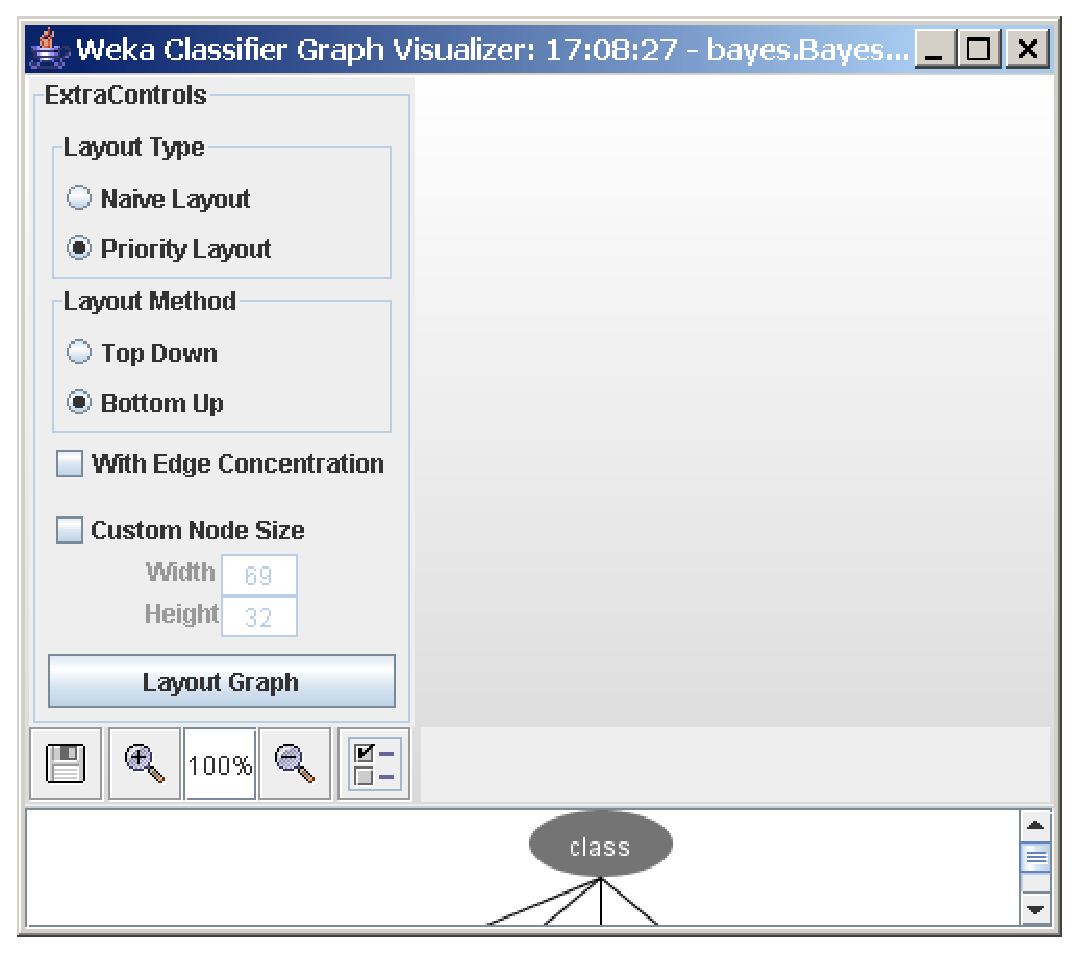
\epsfig{file=images/bayesnet/gui.netoptions.eps,height=7cm}
\end{center}

The {\tt Layout Type} determines the algorithm applied to place the nodes.

The {\tt Layout Method} determines in which direction nodes are considered.

The {\tt Edge Concentration} toggle allows edges to be partially merged.

The {\tt Custom Node Size} can be used to override the automatically determined node size.

When you click a node in the Bayesian net, a window with the probability table of the node 
clicked pops up. The left side shows the parent attributes and lists the values of the
parents, the right side shows the probability of the node clicked conditioned on the 
values of the parents listed on the left.

\begin{center}
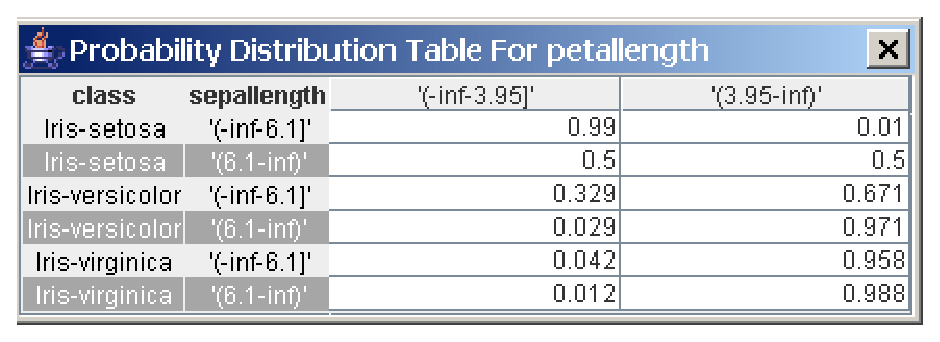
\epsfig{file=images/bayesnet/gui.table.eps,height=3cm}
\end{center}

So, the graph visualizer allows you to inspect both network structure and probability tables. 

\section{Bayes Network GUI}

The Bayesian network editor is a stand alone application with the following features\\
$\bullet$ Edit Bayesian network completely by hand, with unlimited undo/redo stack,
cut/copy/paste and layout support.\\
$\bullet$ Learn Bayesian network from data using learning algorithms in Weka.\\
$\bullet$ Edit structure by hand and learn conditional probability tables (CPTs) using learning algorithms in Weka.\\
$\bullet$ Generate dataset from Bayesian network.\\
$\bullet$ Inference (using junction tree method) of evidence through the network,
interactively changing values of nodes.\\
$\bullet$ Viewing cliques in junction tree.\\
$\bullet$ Accelerator key support for most common operations.\\


The Bayes network GUI is started as\\
java weka.classifiers.bayes.net.GUI <bif file> \\
The following window pops up when an XML BIF file is specified (if none is
specified an empty graph is shown).

\begin{center}
\epsfig{file=images/bayesnet.editor/viewgraph.eps,height=12cm}
\end{center}


\subsubsection*{Moving a node}
Click a node with the left mouse button and drag the node to the desired position.

\subsubsection*{Selecting groups of nodes}

Drag the left mouse button in the graph panel. A rectangle is shown and
all nodes intersecting with the rectangle are selected when the mouse is
released. Selected nodes are made visible with four little black squares at the 
corners (see screenshot above).

The selection can be extended by keeping the shift key pressed while selecting
another set of nodes.

The selection can be toggled by keeping the ctrl key pressed. All nodes in the
selection selected in the rectangle are de-selected, while the ones not in the
selection but intersecting with the rectangle are added to the selection.

Groups of nodes can be moved by keeping the left mouse pressed on one of the
selected nodes and dragging the group to the desired position.

\subsubsection*{File menu}

\begin{center}

\epsfig{file=images/bayesnet.editor/menufile.eps,height=4cm}
\end{center}

The New, Save, Save As, and Exit menu provide functionality as expected.
The file format used is XML BIF \cite{cozman}.

There are two file formats supported for opening\\
$\bullet$ {\bf .xml} for XML BIF files. The Bayesian network is reconstructed
from the information in the file. Node width information is not stored so the nodes
are shown with the default width. This can be changed by laying out the graph
(menu Tools/Layout).\\
$\bullet$ {\bf .arff} Weka data files. When an arff file is selected, a new
empty Bayesian network is created with nodes for each of the attributes
in the arff file. Continuous variables are discretized using the 
{\tt weka.filters.supervised.attribute.Discretize} filter (see note at end of
this section for more details). The network
structure can be specified and the CPTs learned using the Tools/Learn CPT
menu.

The Print menu works (sometimes) as expected.

The Export menu allows for writing the graph panel to image (currently
supported are bmp, jpg, png and eps formats). This can also be activated
using the Alt-Shift-Left Click action in the graph panel.

\subsubsection*{Edit menu}

\begin{center}
\epsfig{file=images/bayesnet.editor/menuedit.eps,height=8cm}
\end{center}

Unlimited undo/redo support. Most edit operations on the Bayesian network
are undoable. A notable exception is learning of network and CPTs.

Cut/copy/paste support. When a set of nodes is selected these can be placed on
a clipboard (internal, so no interaction with other applications yet) and
a paste action will add the nodes. Nodes are renamed by adding "Copy of" before
the name and adding numbers if necessary to ensure uniqueness of name.
Only the arrows to parents are copied, not these of the children.

The Add Node menu brings up a dialog (see below) that allows to specify the name of the
new node and the cardinality of the new node. Node values are assigned the
names 'Value1', 'Value2' etc. These values can be renamed (right click the node
in the graph panel and select Rename Value). Another option is to copy/paste
a node with values that are already properly named and rename the node.

\begin{center}

\epsfig{file=images/bayesnet.editor/dlg.addnode.eps,height=2.5cm}
\end{center}

The Add Arc menu brings up a dialog to choose a child node first;

\begin{center}

\epsfig{file=images/bayesnet.editor/dlg.addarc.eps,height=2cm}
\end{center}

Then a dialog is shown to select a parent. Descendants of the child
node, parents of the child node and the node itself are not listed since
these cannot be selected as child node since they would introduce cycles
or already have an arc in the network.

\begin{center}

\epsfig{file=images/bayesnet.editor/dlg.addarc2.eps,height=2cm}
\end{center}

The Delete Arc menu brings up a dialog with a list of all arcs that
can be deleted.

\begin{center}

\epsfig{file=images/bayesnet.editor/dlg.delarc.eps,height=2cm}
\end{center}

The list of eight items at the bottom are active only when a group of at least
two nodes are selected.\\
$\bullet$ Align Left/Right/Top/Bottom moves the nodes in the selection such
that all nodes align to the utmost left, right, top or bottom node in the
selection respectively.\\
$\bullet$ Center Horizontal/Vertical moves nodes in the selection halfway
between left and right most (or top and bottom most respectively).\\
$\bullet$ Space Horizontal/Vertical spaces out nodes in the selection evenly
between left and right most (or top and bottom most respectively). The order
in which the nodes are selected impacts the place the node is moved to.\\

\subsubsection*{Tools menu}

\begin{center}

\epsfig{file=images/bayesnet.editor/menutools.eps,height=5cm}
\end{center}


The Generate Network menu allows generation of a complete random Bayesian 
network. It brings up a dialog to specify the number of nodes, number of
arcs, cardinality and a random seed to generate a network.

\begin{center}

\epsfig{file=images/bayesnet.editor/dlg.generate.eps,height=3.5cm}
\end{center}


The Generate Data menu allows for generating a data set from the Bayesian
network in the editor. A dialog is shown to specify the number of instances
to be generated, a random seed and the file to save the data set into. The
file format is arff. When no file is selected (field left blank) no file is 
written and only the internal data set is set.

\begin{center}

\epsfig{file=images/bayesnet.editor/dlg.generated.eps,height=3.5cm}
\end{center}

The Set Data menu sets the current data set. From this data set a new
Bayesian network can be learned, or the CPTs of a network can be estimated.
A file choose menu pops up to select the arff file containing the data.

The Learn Network and Learn CPT menus are only active when a data set is 
specified either through
\\$\bullet$ Tools/Set Data menu, or
\\$\bullet$ Tools/Generate Data menu, or
\\$\bullet$ File/Open menu when an arff file is selected.

The Learn Network action learns the whole Bayesian network from the data set.
The learning algorithms can be selected from the set available in Weka
by selecting the Options button in the dialog below.
Learning a network clears the undo stack.

\begin{center}

\epsfig{file=images/bayesnet.editor/dlg.learn.eps,height=2cm}
\end{center}

The Learn CPT menu does not change the structure of the Bayesian network,
only the probability tables.
Learning the CPTs clears the undo stack.

The Layout menu runs a graph layout algorithm on the network and tries to 
make the graph a bit more readable. When the menu item is selected, the node
size can be specified or left to calculate by the algorithm based on the size
of the labels by deselecting the custom node size check box.

\begin{center}

\epsfig{file=images/bayesnet.editor/dlg.layout.eps,height=3cm}
\end{center}

The Show Margins menu item makes marginal distributions visible.
These are calculated using the junction tree algorithm \cite{lauritzen}.
Marginal probabilities for nodes are shown in green next to the node.
The value of a node can be set (right click node, set evidence, select
a value) and the color is changed to red to indicate evidence is set
for the node. Rounding errors may occur in the marginal probabilities.

\begin{center}
\epsfig{file=images/bayesnet.editor/viewevidence.eps,height=8cm}
\end{center}


The Show Cliques menu item makes the cliques visible that are used
by the junction tree algorithm. Cliques are visualized using colored
undirected edges. Both margins and cliques can be shown at the same time,
but that makes for rather crowded graphs.

\begin{center}
\epsfig{file=images/bayesnet.editor/viewcliques.eps,height=8cm}
\end{center}


\subsubsection*{View menu}
The view menu allows for zooming in and out of the graph panel.
Also, it allows for hiding or showing the status and toolbars.

\begin{center}

\epsfig{file=images/bayesnet.editor/menuview.eps,height=5cm}
\end{center}

\subsubsection*{Help menu}

The help menu points to this document.

\begin{center}

\epsfig{file=images/bayesnet.editor/menuhelp.eps,height=2cm}
\end{center}


\subsubsection*{Toolbar}

\begin{center}

\epsfig{file=images/bayesnet.editor/toolbar.eps, height=0.6cm}
\end{center}

The toolbar allows a shortcut to many functions. Just hover the mouse
over the toolbar buttons and a tooltiptext pops up that tells which 
function is activated. The toolbar can be shown or hidden with the View/View 
Toolbar menu.

\subsubsection*{Statusbar}

At the bottom of the screen the statusbar shows messages. This can be 
helpful when an undo/redo action is performed that does not have any
visible effects, such as edit actions on a CPT. The statusbar can be shown 
or hidden with the View/View Statusbar menu.

\subsubsection*{Click right mouse button}

Clicking the right mouse button in the graph panel outside a node
brings up the following popup menu. It allows to add a node
at the location that was clicked, or add select a parent to
add to all nodes in the selection. If no node is selected, or no node
can be added as parent, this function is disabled.
\begin{center}
\epsfig{file=images/bayesnet.editor/popupmenuleft.eps,height=2.5cm}
\end{center}

Clicking the right mouse button on a node brings up a popup menu.

The popup menu shows list of values that can be set as evidence to selected node.
This is only visible when margins are shown (menu Tools/Show margins).
By selecting 'Clear', the value of the node is removed and the margins
calculated based on CPTs again.
\begin{center}
\epsfig{file=images/bayesnet.editor/pop.r.setevidence.eps,height=6cm}
\end{center}
	
A node can be renamed by right click and select Rename in the popup menu.
The following dialog appears that allows entering a new node name.
\begin{center}

\epsfig{file=images/bayesnet.editor/dlg.renamenode.eps,height=2.5cm}
\end{center}



The CPT of a node can be edited manually by selecting a node,
right click/Edit CPT. A dialog is shown with a table representing the
CPT. When a value is edited, the values of the remainder of the table
are update in order to ensure that the probabilities add up to 1.
It attempts to adjust the last column first, then goes backward from there.
\begin{center}
\epsfig{file=images/bayesnet.editor/dlg.CPT.eps,height=6cm}
\end{center}
The whole table can be filled with randomly generated distributions by
selecting the Randomize button.



The popup menu shows list of parents that can be added to selected node.
CPT for the node is updated by making copies for each value of the new parent.
\begin{center}
\epsfig{file=images/bayesnet.editor/pop.r.addparent.eps,height=6cm}
\end{center}

The popup menu shows list of parents that can be deleted from selected node.
CPT of the node keeps only the one conditioned on the first value of the
parent node.
\begin{center}
\epsfig{file=images/bayesnet.editor/pop.r.delparent.eps,height=6cm}
\end{center}

The popup menu shows list of children that can be deleted from selected node.
CPT of the child node keeps only the one conditioned on the first value 
of the parent node.
\begin{center}
\epsfig{file=images/bayesnet.editor/pop.r.delchild.eps,height=6cm}
\end{center}


Selecting the Add Value from the popup menu brings up this dialog,
in which the name of the new value for the node can be specified.
The distribution for the node assign zero probability to the value.
Child node CPTs are updated by copying distributions conditioned on
the new value.
\begin{center}

\epsfig{file=images/bayesnet.editor/dlg.addvalue.eps,height=2.5cm}
\end{center}

The popup menu shows list of values that can be renamed for selected node.
\begin{center}
\epsfig{file=images/bayesnet.editor/pop.r.renvalue.eps,height=6cm}
\end{center}

Selecting a value brings up the following dialog in which a new name
can be specified.
\begin{center}

\epsfig{file=images/bayesnet.editor/dlg.renamevalue.eps,height=2.5cm}
\end{center}

The popup menu shows list of values that can be deleted from selected node.
This is only active when there are more then two values for the node (single
valued nodes do not make much sense).
By selecting the value the CPT of the node is updated in order to ensure
that the CPT adds up to unity. The CPTs of children are updated by dropping
the distributions conditioned on the value.
\begin{center}
\epsfig{file=images/bayesnet.editor/pop.r.delvalue.eps,height=6cm}
\end{center}


\subsection*{A note on CPT learning}

Continuous variables are discretized by the Bayes network class.
The discretization algorithm chooses its values based on the information
in the data set. However, these values are not stored anywhere. So,
reading an arff file with continuous variables using the File/Open menu
allows one to specify a network, then learn the CPTs from it since the
discretization bounds are still known. However, opening an arff file, specifying
a structure, then closing the application, reopening and trying to learn the
network from another file containing continuous variables may not give the
desired result since a the discretization algorithm is re-applied and new
boundaries may have been found. Unexpected behavior may be the result.

Learning from a dataset that contains more attributes than there are nodes
in the network is ok. The extra attributes are just ignored.

Learning from a dataset with differently ordered attributes is ok. Attributes
are matched to nodes based on name. However, attribute values are matched
with node values based on the order of the values.

The attributes in the dataset should have the same number of values as the
corresponding nodes in the network (see above for continuous variables).

\section{Bayesian nets in the experimenter}

Bayesian networks generate extra measures that can be examined in the experimenter.
The experimenter can then be used to calculate mean and variance for those measures.

The following metrics are generated:
\begin{itemize}
\item measureExtraArcs: extra arcs compared to reference network. The network must be
provided as BIFFile to the BayesNet class. If no such network is provided, this value is zero.
\item measureMissingArcs: missing arcs compared to reference network or zero if not provided.
\item measureReversedArcs: reversed arcs compared to reference network or zero if not provided.
\item measureDivergence: divergence of network learned compared to reference network or zero if not provided.
\item measureBayesScore: log of the K2 score of the network structure.
\item measureBDeuScore: log of the BDeu score of the network structure.
\item measureMDLScore: log of the MDL score.
\item measureAICScore: log of the AIC score.
\item measureEntropyScore:log of the entropy.
\end{itemize}


\section{Adding your own Bayesian network learners}

You can add your own structure learners and estimators.

\subsection*{Adding a new structure learner}

Here is the quick guide for adding a structure learner:

\begin{enumerate}
\item Create a class that derives from {\tt weka.classifiers.bayes.net.search.SearchAlgorithm}.
  If your searcher is score based, conditional independence based or cross-validation based, you
  probably want to derive from {\tt ScoreSearchAlgorithm}, {\tt CISearchAlgorithm} or {\tt CVSearchAlgorithm}
  instead of deriving from {\tt SearchAlgorithm} directly.
  Let's say it is called \\{\tt weka.classifiers.bayes.net.search.local.MySearcher}
  derived from {\tt ScoreSearchAlgorithm}.

\item Implement the method\\
{\tt public void buildStructure(BayesNet bayesNet, Instances instances)}.
Essentially, you are responsible for setting the parent sets in {\tt bayesNet}.
You can access the parentsets using {\tt bayesNet.getParentSet(iAttribute)} where
{\tt iAttribute} is the number of the node/variable.

To add a parent {\tt iParent} to node {\tt iAttribute}, use\\ 
{\tt bayesNet.getParentSet(iAttribute).AddParent(iParent, instances)} where
{\tt instances} need to be passed for the parent set to derive properties of
the attribute.

Alternatively, implement
{\tt public void search(BayesNet bayesNet, Instances instances)}.
The implementation of {\tt buildStructure} in the base class.
This method is called by the {\tt SearchAlgorithm} will call search
after initializing parent sets and if the {\tt initAsNaiveBase} flag is set, it will
start with a naive Bayes network structure. After calling {\tt search} in your
custom class, it will add arrows if the {\tt markovBlanketClassifier} flag is 
set to ensure all attributes are in the Markov blanket of the class node.

\item If the structure learner has options that are not default options,
you want to implement {\tt public Enumeration listOptions()}, 
{\tt public void setOptions(String[] options)}, 
{\tt public String[] getOptions()} and the get and set methods for
the properties you want to be able to set.

NB 1. do not use the -E option since that is reserved for the {\tt BayesNet} class to 
distinguish the extra options for the {\tt SearchAlgorithm} class and the {\tt Estimator} class.
If the -E option is used, it will not be passed to your {\tt SearchAlgorithm} (and
probably causes problems in the {\tt BayesNet} class).

NB 2. make sure to process options of the parent class if any in the get/setOpions
methods.
\end{enumerate}

\subsection*{Adding a new estimator}

This is the quick guide for adding a new estimator:

\begin{enumerate}
\item Create a class that derives from \\
  {\tt weka.classifiers.bayes.net.estimate.BayesNetEstimator}.
  Let's say it is called \\
  {\tt weka.classifiers.bayes.net.estimate.MyEstimator}.

\item Implement the methods\\
{\tt public void initCPTs(BayesNet bayesNet)} \\
{\tt public void estimateCPTs(BayesNet bayesNet)} \\
{\tt public void updateClassifier(BayesNet bayesNet, Instance instance)}, and \\
{\tt  public double[] distributionForInstance(BayesNet bayesNet, Instance instance)}.

\item If the structure learner has options that are not default options,
you want to implement {\tt public Enumeration listOptions()},
{\tt public void setOptions(String[] options)},
{\tt public String[] getOptions()} and the get and set methods for
the properties you want to be able to set.

NB do not use the -E option since that is reserved for the BayesNet class to 
distinguish the extra options for the SearchAlgorithm class and the Estimator class.
If the -E option is used and no extra arguments are passed to the SearchAlgorithm,
the extra options to your Estimator will be passed to the SearchAlgorithm
instead. In short, do not use the -E option.
\end{enumerate}

\section{FAQ}

\subsection*{How do I use a data set with continuous variables with the BayesNet classes?}
Use the class {\tt weka.filters.unsupervised.attribute.Discretize} to discretize them.
From the command line, you can use\\
{\tt java weka.filters.unsupervised.attribute.Discretize -B 3 -i infile.arff -o outfile.arff}\\
where the -B option determines the cardinality of the discretized variables.

\subsection*{How do I use a data set with missing values with the BayesNet classes?}
You would have to delete the entries with missing values or
fill in dummy values.

\subsection*{How do I create a random Bayes net structure?}

Running from the command line \\
{\tt java  weka.classifiers.bayes.net.BayesNetGenerator -B -N 10 -A 9 -C 2}\\
will print a Bayes net with 10 nodes, 9 arcs and binary variables
in XML BIF format to standard output.

\subsection*{How do I create an artificial data set using a random Bayes nets?}
Running\\
{\tt java  weka.classifiers.bayes.net.BayesNetGenerator -N 15 -A 20 -C 3 -M 300}\\
will generate a data set in arff format with 300 instance from a random
network with 15 ternary variables and 20 arrows.

\subsection*{How do I create an artificial data set using a Bayes nets I have on file?}
Running\\
{\tt java  weka.classifiers.bayes.net.BayesNetGenerator -F alarm.xml -M 1000}\\
will generate a data set with 1000 instances from the network stored in the file
{\tt alarm.xml}.

\subsection*{How do I save a Bayes net in BIF format?}
\begin{itemize}
\item {\bf GUI:} In the Explorer
\begin{itemize}
\item learn the network structure,
\item right click the relevant run in the result list,
\item choose ``Visualize graph'' in the pop up menu,
\item click the floppy button in the Graph Visualizer window.
\item a file ``save as'' dialog pops up that allows you to select the file name to save to.
\end{itemize}

\item {\bf Java:} Create a {\tt BayesNet} and call {\tt BayesNet.toXMLBIF03()}
which returns the Bayes network in BIF format as a String.

\item {\bf Command line:} use the {\tt -g} option and redirect the output on stdout into a file.
\end{itemize}

\subsection*{How do I compare a network I learned with one in BIF format?}
Specify the -B $<$bif-file$>$ option to BayesNet. 
Calling {\tt toString()} will produce a summary of extra, missing and reversed arrows.
Also the divergence between the network learned and the one on file is reported.

\subsection*{How do I use the network I learned for general inference?}
There is no general purpose inference in Weka, but you can export the
network as XML BIF file (see above) and import it in other packages,
for example JavaBayes available under GPL from
\url{http://www.cs.cmu.edu/\~javabayes}{}.


\section{Future development}

If you would like to add to the current Bayes network facilities in Weka, you might
consider one of the following possibilities.

\begin{itemize}
\item Implement more search algorithms, in particular, 
\begin{itemize}
\item general purpose search algorithms (such as an improved implementation of 
genetic search).
\item structure search based on equivalent model classes.
\item implement those algorithms both for local and global metric based search algorithms.
\item implement more conditional independence based search algorithms.
\end{itemize}

\item Implement score metrics that can handle sparse instances in order to allow 
for processing large datasets.

\item Implement traditional conditional independence tests for conditional
independence based structure learning algorithms.

\item Currently, all search algorithms assume that all variables are discrete.
Search algorithms that can handle continuous variables would be interesting.

\item A limitation of the current classes is that they assume that there
are no missing values. This limitation can be undone by implementing score metrics 
that can handle missing values.
The classes used for estimating the conditional probabilities need to be updated
as well.

\item Only leave-one-out, k-fold and cumulative cross-validation are implemented.
These implementations can be made more efficient and other cross-validation methods
can be implemented, such as Monte Carlo cross-validation and bootstrap cross
validation.

\item Implement methods that can handle incremental extensions of the data set for
updating network structures.

\end{itemize}

And for the more ambitious people, there are the following challenges.

\begin{itemize}
\item A GUI for manipulating Bayesian network to allow user intervention for
adding and deleting arcs and updating the probability tables.

\item General purpose inference algorithms built into the GUI to allow user
defined queries.

\item Allow learning of other graphical models, such as chain graphs,
undirected graphs and variants of causal graphs.

\item Allow learning of networks with latent variables.

\item Allow learning of dynamic Bayesian networks so that time series data
can be handled.
\end{itemize}
